% Work-MAT -- 2. rocnik, hodina 08. Zaporne celociselne exponenty.
\documentclass[11pt,a4paper]{article}
\input{../../sablony/pripravy/priprava.sty}
\usepackage{tikz}
\usetikzlibrary{arrows.meta}
\nastavPripravu{2. ročník}{Mocninné funkce}{08}{Mocninné funkce II: záporné exponenty}
\begin{document}
\poznamka{Doporučené jádro: přepis pomocí zlomku 7 min, definiční obor 7 min, dvojice grafů 12 min, asymptoty 8 min, samostatná práce 8 min, uzavření 3 min. Funkce $x^{-n}$ není definovaná v nule. Znaménko a obor hodnot odvozujte z parity $n$.}

\blok{Záporný exponent znamená převrácenou hodnotu}
V prvním ročníku jsme zavedli mocniny se záporným exponentem. Připomeňme si pravidlo $x^{-n}=1/x^n$ pro $x\ne0$. Nyní jej použijeme pro funkce.

\begin{definiceBox}[title={Definice - Mocninná funkce se záporným celočíselným exponentem}]
Pro přirozené číslo $n\ge1$ je funkce s předpisem
\[
f(x)=x^{-n}=\frac{1}{x^n},\qquad D(f)=\mathbb R\setminus\{0\},
\]
mocninnou funkcí se záporným celočíselným exponentem.
\end{definiceBox}

\begin{prikladReseniBox}[title={Příklad 1}]
Doplň hodnoty funkcí $f(x)=x^{-2}$ a $g(x)=x^{-3}$ pro $x\in\{-2;-1;1;2\}$. Rozhodni, která je sudá a která lichá.
\tcblower
\[
\begin{array}{c|rrrr}
x&-2&-1&1&2\\\hline
f(x)=\frac{1}{x^2}&\frac{1}{4}&1&1&\frac{1}{4}\\
g(x)=\frac{1}{x^3}&-\frac{1}{8}&-1&1&\frac{1}{8}
\end{array}
\]
Platí $f(-x)=f(x)$, tedy $f$ je sudá. Naproti tomu $g(-x)=-g(x)$, takže $g$ je lichá.
\end{prikladReseniBox}

\begin{center}
\begin{minipage}{.47\linewidth}\centering
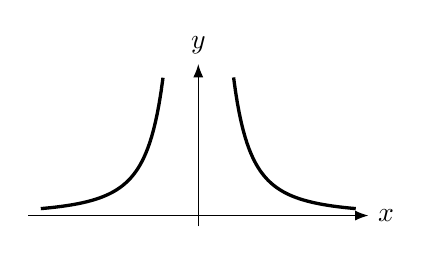
\begin{tikzpicture}[x=.8cm,y=.55cm,>=Latex]
\draw[->](-2.7,0)--(2.7,0)node[right]{$x$};\draw[->](0,-.25)--(0,3.5)node[above]{$y$};
\draw[very thick,domain=-2.5:-.56,samples=65]plot(\x,{1/(\x*\x)});
\draw[very thick,domain=.56:2.5,samples=65]plot(\x,{1/(\x*\x)});
\end{tikzpicture}\par\footnotesize $x^{-2}$: dvě větve nad osou $x$
\end{minipage}\hfill
\begin{minipage}{.47\linewidth}\centering
\begin{tikzpicture}[x=.8cm,y=.55cm,>=Latex]
\draw[->](-2.7,0)--(2.7,0)node[right]{$x$};\draw[->](0,-3.5)--(0,3.5)node[above]{$y$};
\draw[very thick,domain=-2.5:-.66,samples=65]plot(\x,{1/(\x*\x*\x)});
\draw[very thick,domain=.66:2.5,samples=65]plot(\x,{1/(\x*\x*\x)});
\end{tikzpicture}\par\footnotesize $x^{-3}$: větve v I. a III. kvadrantu
\end{minipage}
\end{center}

\begin{definiceBox}[title={Definice - Asymptota grafu}]
\textbf{Asymptota} je přímka, ke které se část grafu neomezeně přibližuje. U funkcí $f(x)=x^{-n}$ je \textbf{svislou asymptotou} přímka $x=0$ a \textbf{vodorovnou asymptotou} přímka $y=0$.
\end{definiceBox}
\poznamka{Asymptotu vysvětluj zatím intuitivně pomocí grafu a hodnot v tabulce, nikoli přes limity. Funkce $x^{-n}$ nenabývají hodnoty $0$ a nejsou definovány pro $x=0$.}

\begin{zadaniBox}[title={Věta - Parita a obor hodnot záporných mocnin}]
Pro $f(x)=x^{-n}$, $n\ge1$, je $D(f)=\mathbb R\setminus\{0\}$. Pro sudé $n$ je funkce sudá a $H(f)=(0;+\infty)$. Pro liché $n$ je funkce lichá a $H(f)=\mathbb R\setminus\{0\}$.
\end{zadaniBox}
\noindent\textbf{Zdůvodnění.}\enspace Je-li $n$ sudé, $x^n>0$ pro $x\ne0$, a převrácená hodnota je kladná. Je-li $n$ liché, $1/x^n$ zachovává znaménko nenulového $x$. Souměrnost plyne z $(-x)^n=(-1)^nx^n$.


\begin{prikladReseniBox}[title={Příklad 2}]
U $f(x)=x^{-4}$ urči $D$, $H$, sudost, znaménko a průsečíky s osami.
\tcblower
$D(f)=\mathbb R\setminus\{0\}$, $H(f)=(0;+\infty)$; je sudá a na celém svém oboru kladná. Nemá průsečík s osou $x$ (nikdy není rovna nule) ani s osou $y$ (v nule není definována).
\end{prikladReseniBox}

\begin{prikladReseniBox}[title={Příklad 3}]
Pro $h(x)=-\frac{3}{x^2}$ urči definiční obor, obor hodnot, paritu, asymptoty a funkční hodnoty $h(-1)$, $h(1)$, $h(2)$.
\tcblower
$D(h)=\mathbb R\setminus\{0\}$ a $H(h)=(-\infty;0)$. Funkce je sudá, protože $h(-x)=h(x)$. Asymptoty jsou $x=0$ a $y=0$. Platí $h(-1)=h(1)=-3$ a $h(2)=-\frac{3}{4}$. Obě větve leží pod osou $x$.
\end{prikladReseniBox}

\blok{Samostatná práce}
\begin{zadaniReseniBox}[title={Samostatná práce 1}]
\begin{enumerate}[label=\alph*)]
\item Přepiš $x^{-5}$ zlomkem a určete jeho $D$, $H$ a paritu.
\item Urči hodnoty $f(-2)$ a $f(\frac{1}{2})$ pro $f(x)=x^{-2}$.
\item Napiš asymptoty grafu funkce $g(x)=-\frac{2}{x^3}$.
\end{enumerate}
\tcblower
\begin{enumerate}[label=\alph*)]
\item $x^{-5}=1/x^5$, $D=H=\mathbb R\setminus\{0\}$, lichá.
\item $f(-2)=\frac{1}{4}$, $f(\frac{1}{2})=4$.
\item $x=0$, $y=0$. Znaménko $g(x)$ je opačné než znaménko $x$.
\end{enumerate}
\end{zadaniReseniBox}

\begin{zadaniReseniBox}[title={Samostatná práce 2}]
\begin{enumerate}[label=\alph*)]
\item U $f(x)=x^{-4}$ urči $D$, $H$, paritu a asymptoty.
\item U $g(x)=-\frac{2}{x^3}$ urči $D$, $H$, paritu, asymptoty a znaménko na záporných $x$.
\item Pro $p(x)=\frac{1}{2x^2}$ spočítej $p(-2)$, $p(2)$ a popiš polohu grafu vůči osám.
\item Porovnej znaménka $x^{-2}$ a $x^{-3}$ na intervalu $(-\infty;0)$ a vysvětli proč.
\end{enumerate}
\tcblower
\begin{enumerate}[label=\alph*)]
\item $D(f)=\mathbb R\setminus\{0\}$, $H(f)=(0;+\infty)$; sudá, asymptoty $x=0$, $y=0$.
\item $D(g)=H(g)=\mathbb R\setminus\{0\}$; lichá, asymptoty $x=0$, $y=0$. Pro $x<0$ je $g(x)>0$.
\item $p(-2)=p(2)=\frac{1}{8}$. Graf je souměrný podle osy $y$, leží nad osou $x$ a ani jednu osu neprotíná.
\item Pro $x<0$ platí $x^{-2}=\frac{1}{x^2}>0$, ale $x^{-3}=\frac{1}{x^3}<0$, protože sudá mocnina je kladná a lichá zachovává znaménko základu.
\end{enumerate}
\end{zadaniReseniBox}

\begin{zadaniReseniBox}[title={Rozšíření 1}]
Pro funkci $h(x)=1/(x-2)^2$ urči definiční obor, obor hodnot a asymptoty.
\tcblower
$D(h)=\mathbb R\setminus\{2\}$, $H(h)=(0;+\infty)$. Svislá asymptota je $x=2$, vodorovná $y=0$.
\end{zadaniReseniBox}

\begin{zadaniReseniBox}[title={Domácí úkol}]
\textbf{Mix učiva o inverzích, kladných a záporných mocninách:}
\begin{enumerate}[label=\alph*)]
\item U $f(x)=x^{-6}$ a $g(x)=x^{-7}$ urči $D$, $H$, paritu a znaménko pro $x<0$.
\item Vypočítej $2^{-3}$ a $(-2)^{-3}$ a vysvětli rozdíl.
\item Urči inverzi k lineární funkci $h(x)=3x-5$.
\item Urči inverzi k lineárně lomené funkci $k(x)=\frac{x+1}{x-2}$ a její definiční obor.
\item Urči inverzi k $m(x)=(x-1)^2$ na $D(m)=\langle1;+\infty)$.
\item Urči $D$, $H$, paritu a monotónnost funkce $p(x)=x^5$.
\item Urči $D$, $H$, paritu a asymptoty funkce $q(x)=x^{-4}$.
\item Urči $D$, $H$, paritu, znaménko a asymptoty funkce $r(x)=-\frac{2}{x^3}$.
\end{enumerate}
\tcblower
\begin{enumerate}[label=\alph*)]
\item Obě mají $D=\mathbb R\setminus\{0\}$. $x^{-6}$ je sudá, kladná a má $H=(0;+\infty)$; $x^{-7}$ je lichá, pro $x<0$ záporná a má $H=\mathbb R\setminus\{0\}$.
\item $2^{-3}=\frac{1}{8}$, $(-2)^{-3}=-\frac{1}{8}$; třetí mocnina zachovává znaménko základu.
\item
\(\displaystyle\begin{aligned}h(x)&=3x-5 &&\bigm|\ x\to y\\x&=3y-5\\3y&=x+5\\y&=\frac{x+5}{3}\\h^{-1}(x)&=\frac{x+5}{3}\end{aligned}\)
\item
\(\displaystyle\begin{aligned}k(x)&=\frac{x+1}{x-2} &&\bigm|\ x\to y\\x&=\frac{y+1}{y-2}\\x(y-2)&=y+1\\xy-2x&=y+1\\y(x-1)&=2x+1\\y&=\frac{2x+1}{x-1}\\k^{-1}(x)&=\frac{2x+1}{x-1}\end{aligned}\)

$D(k^{-1})=\mathbb R\setminus\{1\}$.
\item
\(\displaystyle\begin{aligned}m(x)&=(x-1)^2 &&\bigm|\ x\to y\\x&=(y-1)^2\\y-1&=\sqrt{x}\\y&=1+\sqrt{x}\\m^{-1}(x)&=1+\sqrt{x}\end{aligned}\)

$D(m^{-1})=\langle0;+\infty)$.
\item $D(p)=H(p)=\mathbb R$; funkce je lichá a přísně roste.
\item $D(q)=\mathbb R\setminus\{0\}$, $H(q)=(0;+\infty)$; sudá, asymptoty $x=0$ a $y=0$.
\item $D(r)=H(r)=\mathbb R\setminus\{0\}$; lichá, pro $x>0$ záporná a pro $x<0$ kladná, asymptoty $x=0$ a $y=0$.
\end{enumerate}
\end{zadaniReseniBox}
\end{document}
